\documentclass[landscape]{slides}

\usepackage[latin1]{inputenc}
\usepackage[T1]{fontenc}
\usepackage{eurosym}
\usepackage[portuguese]{babel}

\usepackage{graphicx}
\usepackage{epsfig,color}
\usepackage{hyperref}
\usepackage{multimedia}

% Remove page numbers
\usepackage{nopageno}

\author{Marcos Marado, \url{https://tilde.pt/~marado}}
% \title{I \heart Free Software!}
\title{
\includegraphics{ilovefs-sticker_thumb.png}}
\date{14 February 2023}

\begin{document}

% TITLE

\begin{slide}
\maketitle
\end{slide}

% CONTENT

\begin{slide}
I

% https://twitter.com/mind_booster/status/1615492561598021635
\center{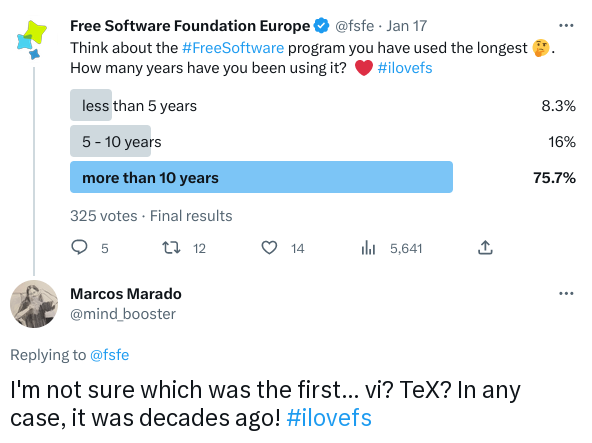
\includegraphics{vim-tex-love.png}}
\end{slide}

\begin{slide}
(But not just I)

% CC0 image from https://download.fsfe.org/campaigns/ilovefs/gallery/ilovefs-gallery-6.jpg
\center{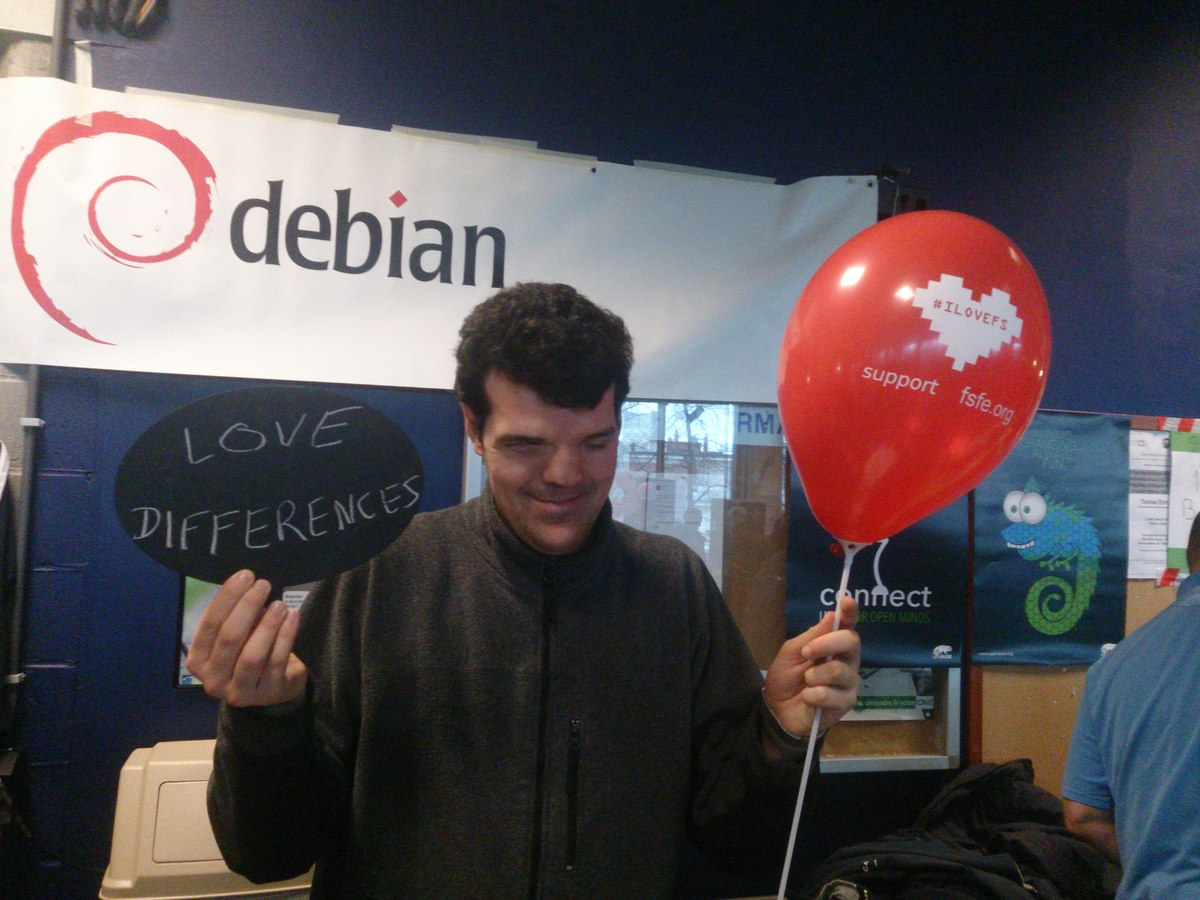
\includegraphics[scale=0.45]{ilovefs-gallery-6.jpg}}
\end{slide}

\begin{slide}
Me and Free Software
  \begin{itemize}
    \item{} user
      \begin{itemize}
          \item{} still VIM and \TeX (for this presentation, for eg.!)
          \item{} Debian and Ubuntu; Android
      \end{itemize}
    \item{} creator
      \begin{itemize}
        \item{} professionally and otherwise
      \end{itemize}
    \item{} community member
      \begin{itemize}
        \item{} ANSOL, the Portuguese FSFE sister organization
      \end{itemize}
  \end{itemize}
\end{slide}

%% 3 - ANSOL (includes explanation about Free Software) - TODO: translate
\input{ANSOL.tex}

%% 4 - Love // I Love Free Software: the campain, how it has been celebrated the last few years % TODO

%% 5 - Videos? (if there's time, and audio) https://media.fsfe.org/w/p/u3Ep8hRP5vFdbgUE9LKScW % TODO

%% Questions?
\begin{slide}
\center{\Huge{QUESTIONS?}}

\url{https://tilde.pt/~marado} \\
\url{http://ansol.org} \\
\url{https://ilovefs.org} \\
\url{http://fsfe.org} \\
\url{http://fsf.org} \\
\url{https://github.com/marado/ilovefs-presentation}
\end{slide}

\end{document}
